\chapter{Study 2: User Study}

Following the first study (See Chapter \ref{ch: chapter 3}), A laboratory study was conducted to evaluate user experience on different design patterns of music sequencers. Base on the previous work of evaluating music instruments, a questionnaire was designed to measure muscians experience (See Section \ref{subsec: questionnaire}).

\section{Method}
\subsection{Questionnaire}
\label{subsec: questionnaire}

Base on \citeauthor{Reference0}'s work, which developed a 80-item pool ordered by descending mean importance for questionnaire, 10 questions that scored the highest mark from 9 different categories were used in the user study (see Appendix \ref{app:Appendix A}).

\citeauthor{Reference0} indicated the following three criteria for musicians to perceive musical instruments:
\begin{flushleft}
  \qquad \qquad \quad\textbf{Experienced freedom and possibilities (EFP)}\\
  \qquad \qquad \quad\textbf{Perceived control and comfort (PCC)} \\
  \qquad \qquad \quad\textbf{Perceived stability, sound quality and aesthetics (PSSQA)}\\
\end{flushleft}
\textit{EFP} as the predominent facet, mainly targets at evaluating the musicianship and expressivity of music instruments. For example, questions like\textit{\textquotedblleft{The instrument allows me to express myself.}\textquotedblright} are used to decide whether the instruments can let muscians to express themselves; \textit{PCC} is used to assess the controbility of the music instruments. Questions such as \textit{\textquotedblleft{I can control the sound appropriately.}\textquotedblright} are setted to identify how well the musicians believed they can control the instruments; \textit{PSSQA} is the most unique facet which analyses the quality of the instruments from the material, the sound and the apperience perspectives. For instance, questions like\textit{\textquotedblleft The instrument pleases me sound-wise\textquotedblright} test the sound quality of the instrument. The above three interrelated facets construct the framework of MPX-Q questionnaire.

\begin{table}
  \caption{Items in the questionnaire with thier factor and category(ordered by descending mean importance)}
  \label{tab: questionnaire}

  \begin{tabular}{ |p{1.2cm}|p{2.5cm}|p{9.2cm}|p{0.6cm}|}
   \multicolumn{4}{l}{} \\
   \hline
   Factor & Category  & Item  & $\mu$ \\
   \hline
   EFP & Creativity & The instrument allows me to be creative & 6.25\\
   & Enjoyment &  I have fun playing the instrument & 6.08\\
   & Expressiveness & The instrument allows me to express myself & 6.06\\
   \hline
   PCC & Conformance & The instrument responds well to my actions & 6.23\\
   & Control & I can control the sound appropriately & 6.04\\
   & Engagement & The instrument allows me to be engaged when I'm playing it & 5.98\\
   & Engagement & I feel the urge to play the instrument again & 5.79\\
   & Play Comfort & I can recognize that the instrument responds well to my playing & 5.85\\
   \hline
   PSSQA & Stability & I can rely on the instrument when playing it & 6.21\\
   & Sound Quality & The instrument pleases me sound-wise & 6.02\\
   \hline
  \end{tabular}
  \small should be a caption
\end{table}

\bigskip

Follow the framework of MPQ-Q questionnaire, 10 questions from 3 factors were implemented in our questionnaire(see Table \ref{tab: questionnaire}). For each factor, only the items score the highest mean importance value in the certain category were picked. Under the EFP factor, we focused at the creativity, enjoyment and expressiveness of the music sequencer. The reason for this, it's because we want to figure out whether the design of the interface is encouraging musicians to explore new possibilities and inspiring musicians' creativity. As for the PCC, items associate with conformance, control and engagement are chose. The reason behind this is when musicians performing on instruments there are a lot of physical interaction between musicians and instruments, whether the musiciain feel conformance and engagement have impact on their overall satisfaction. For items under PSSQA, we only look at the stability and sound quality. Because the more stable of the music sequencer the more confident musicians can rely on it. Same with the sound quality, only the instrument that can satisfy the muscian is able to please the audience.

\subsection{Participants}

In total, twenty participants with different music background were invited and took part in the user study. Fifteen of them are male and five are female. All the participants have at least one year training on music and master at least one instrument. Two participants are semi-professional musicians who have spend more than 10 years on performing and music making. One are currently teaching music in the middle school. The remaining musicians play musical instruments mainly because their parents forced them to do when they were children, however, they were all greatful that they have learned music and still practise the instrument in their spare time.

\bigskip
\begin{figure}[h]
  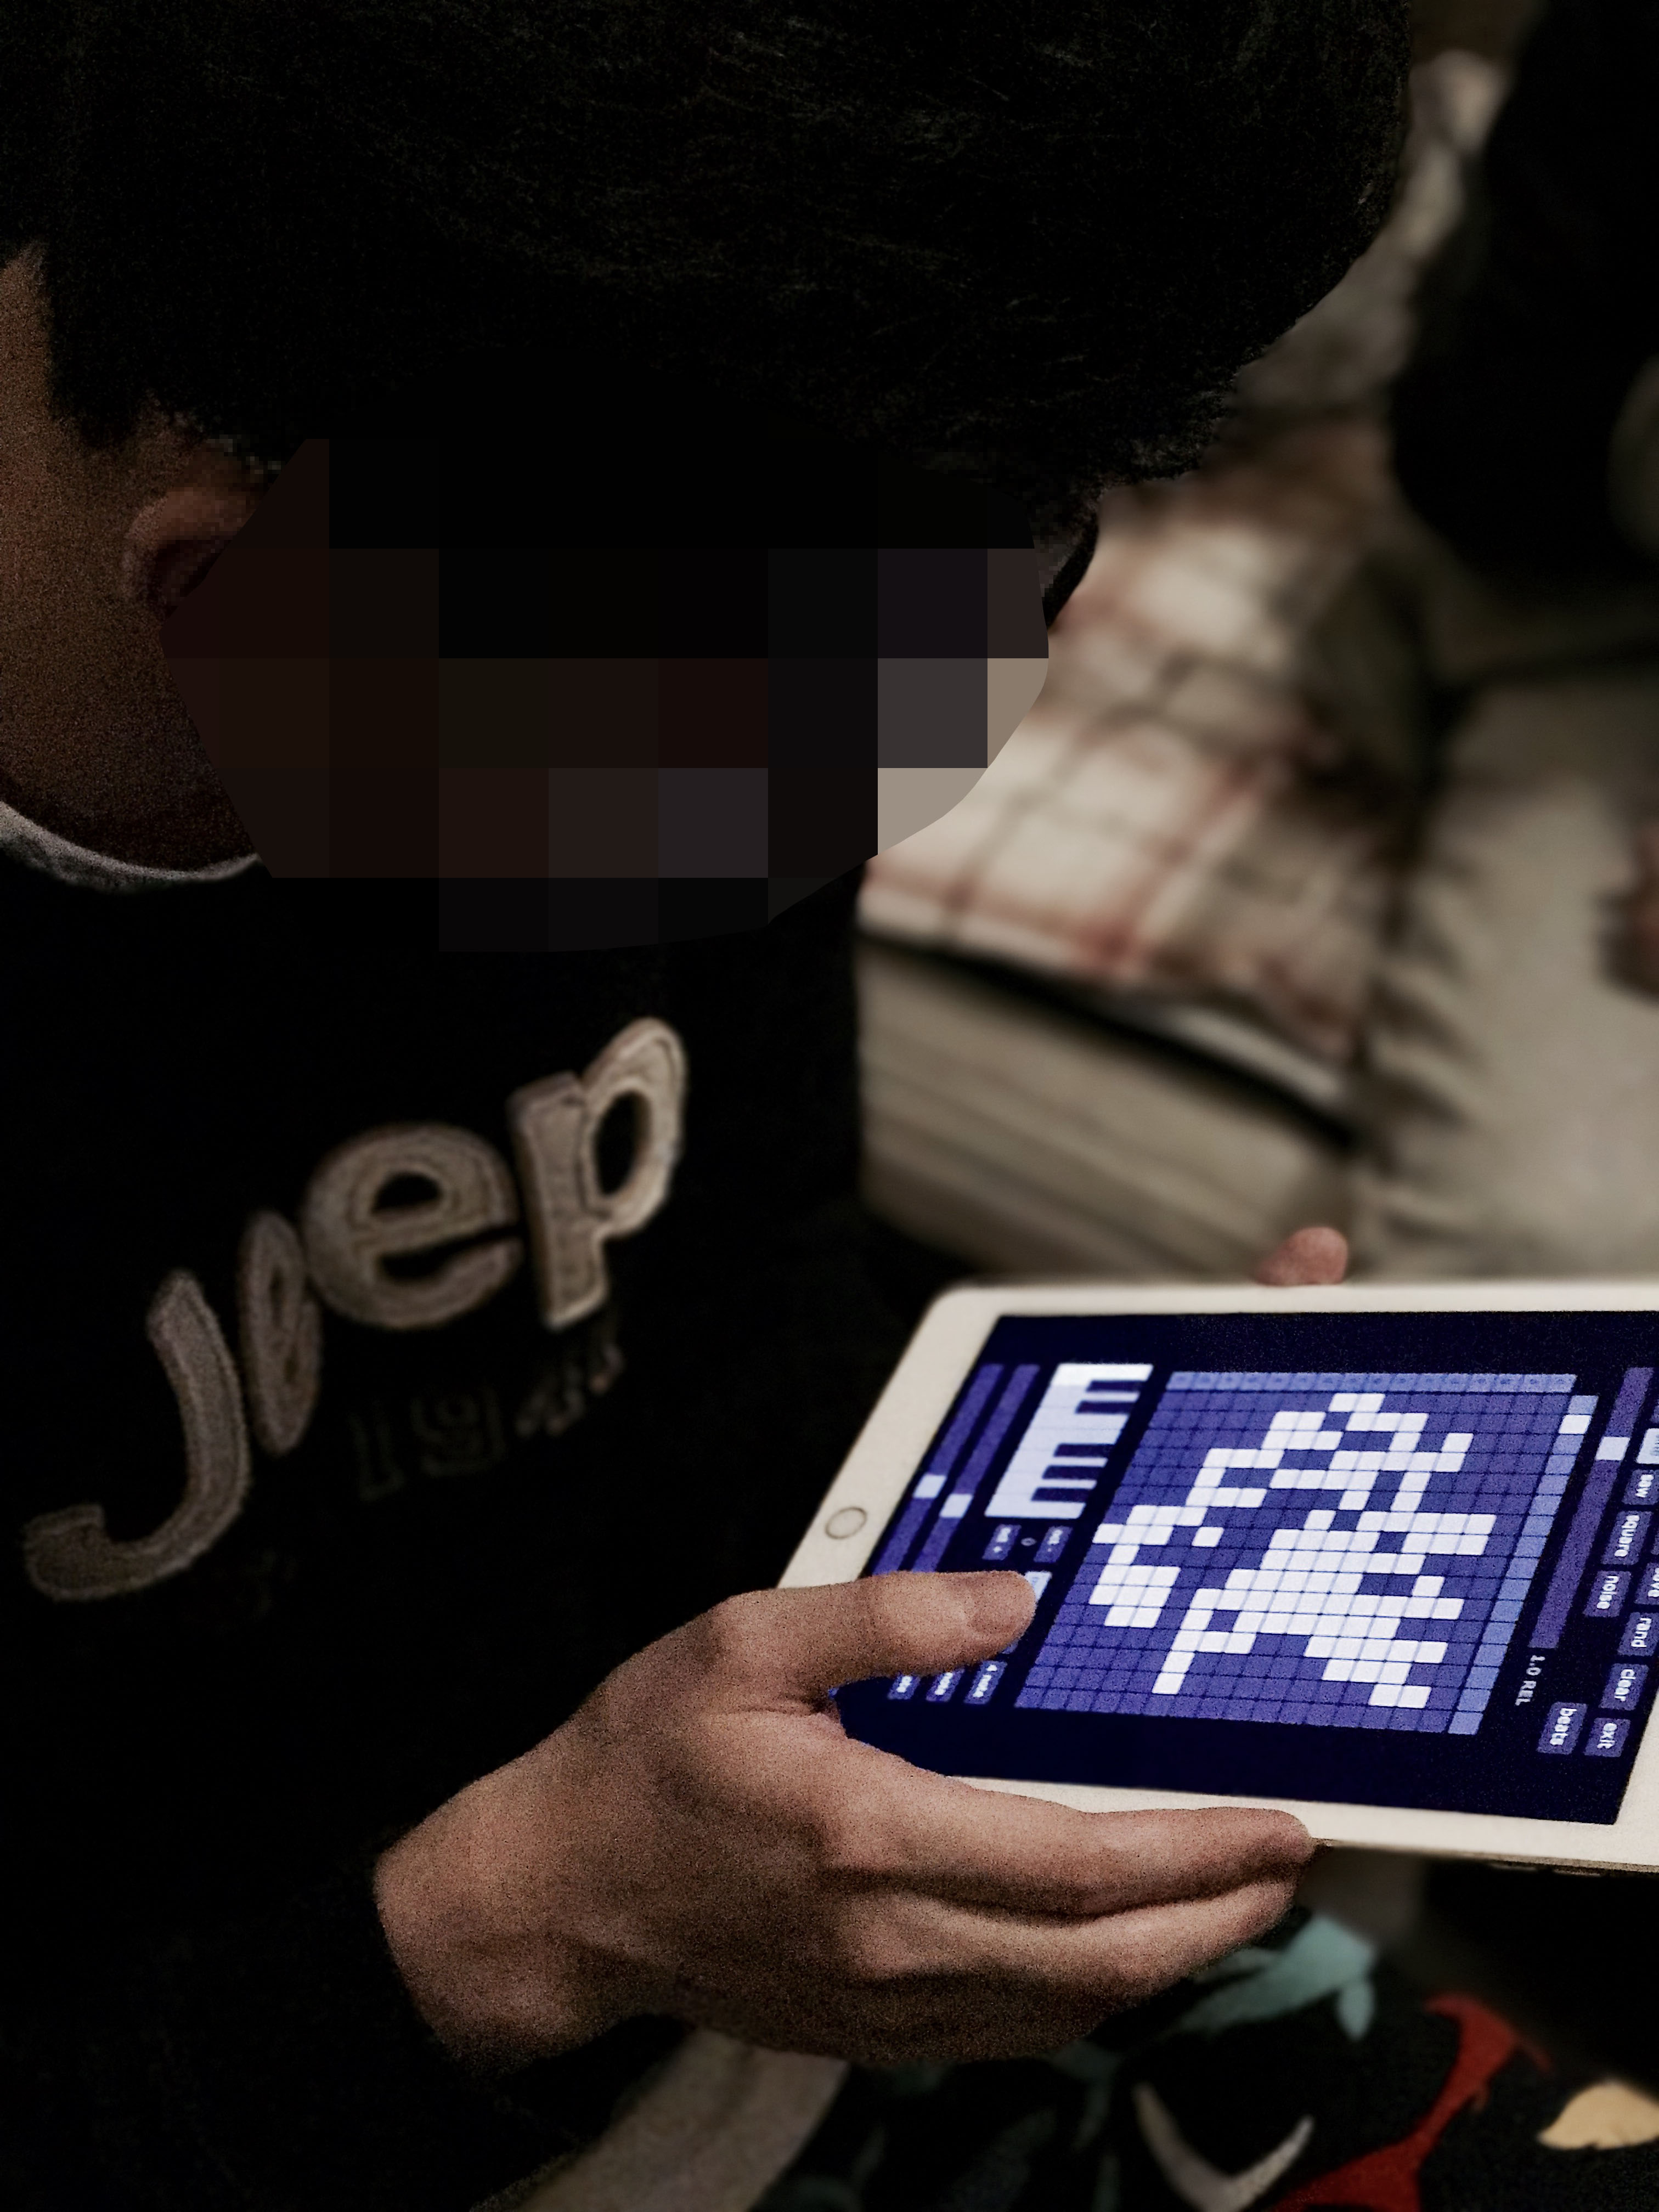
\includegraphics[width=6cm]{images/Participant}
  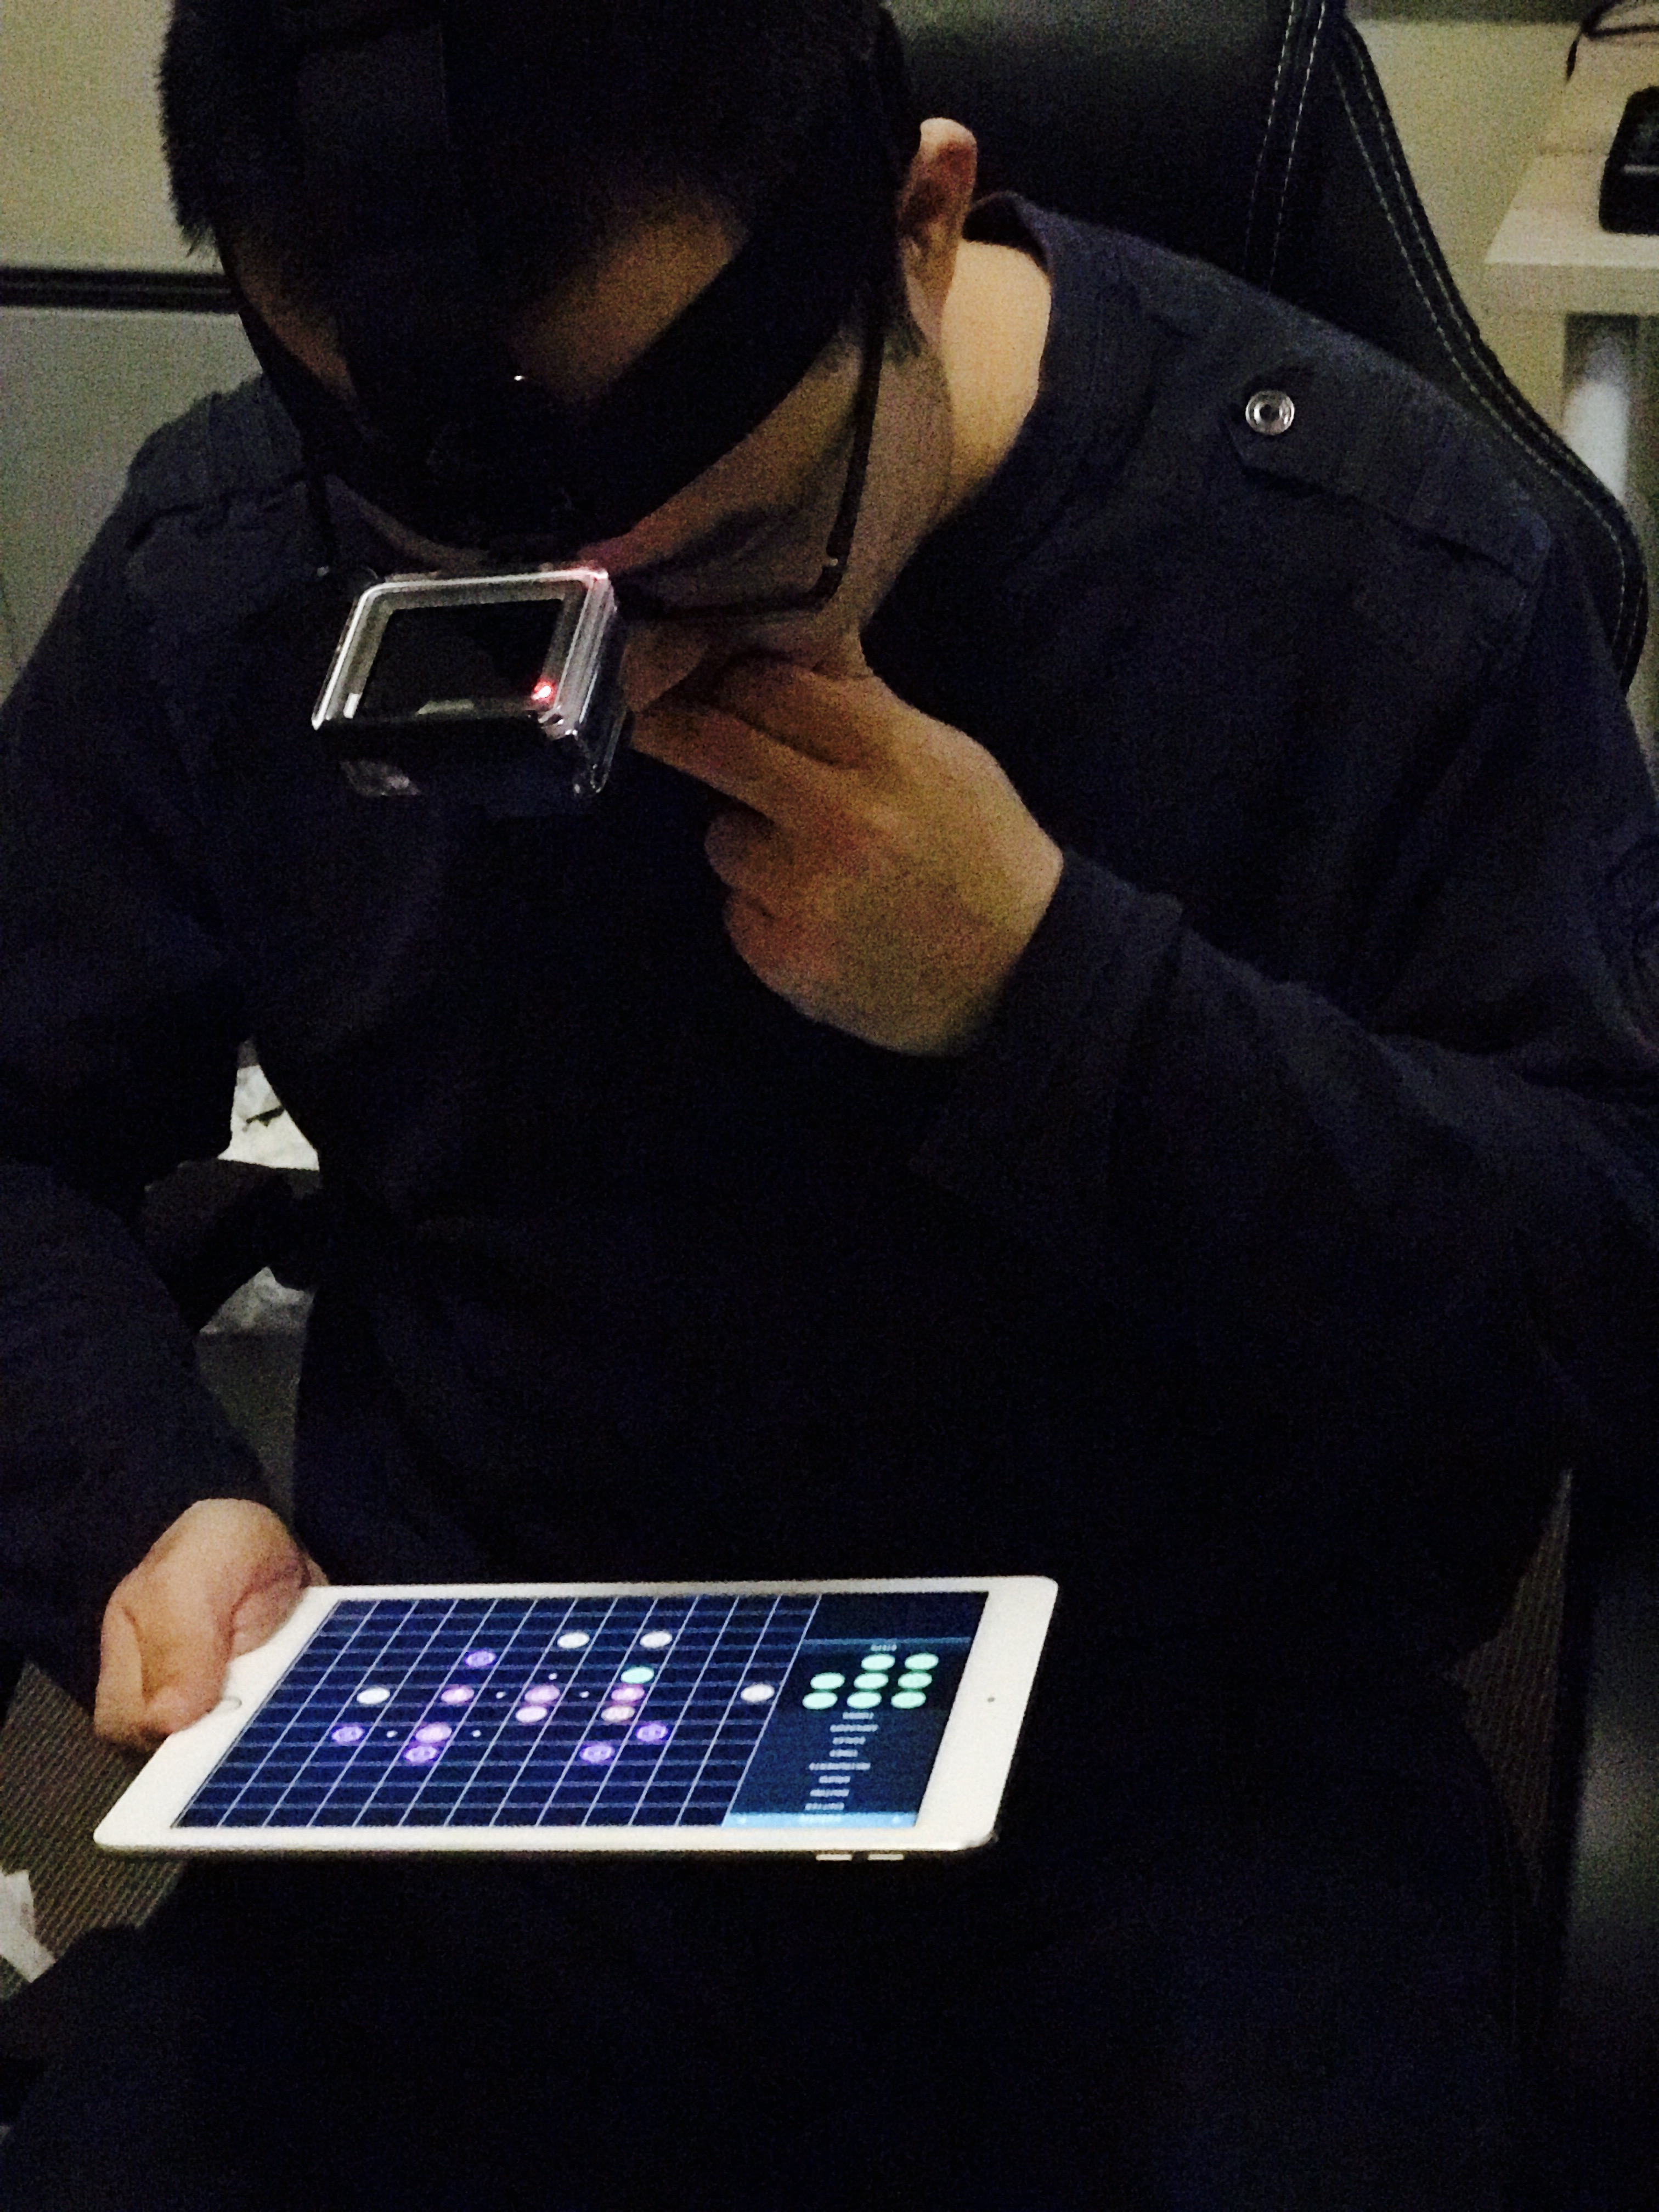
\includegraphics[width=6cm]{images/Participant2}
  \centering
  \caption{Participants test on the music sequencer on iPad}
  \label{fig: participant}
\end{figure}
\bigskip


Four of them have learned more than one instrument. One have learned more than five different instruments. The popular pick of instruments are piano and guitar. Ten participants have learned to play piano and three of them have over five years experience. Seven participants have learned guitar and still play guitar occasionnally. Other instruments are drums, violin and flute. Three participants have experience playing drums. Two have learned to play violin. Two have learned some flute many years ago. But only 15\% had experience on electronic music before and had played on music sequencer on the laptop.

\subsection{Interview}

Participants were intervied at the end of the user study. The main purpose of the interview is to find out the reason behind their decision on the questionnaire. Besides, the music background of participants such as \textit{\textquotedblleft{how many years of music training}\textquotedblright} were recorded for further analysis.

In order to acquire the deeper reason, all the interview followed the same procedure: 1) Since the majority of the participants did not know music sequencer before, they were asked to describe the similarities among the three different music sequencer applications, and then defined what is music sequencer. which was designed to help them to form a general idea of music sequencer. 2) After that, interviewees were asked to choose their favourite application based on different scenario. Also, the interviewee needed to give reasons why certain music sequencer application was better than another. 3) In the final step, all the questions shifted to an abstract level, where they were asked whether music sequencer application on iPad were an instrument ,and what features that made them thought it is or it is not an instrument.

The interviews were recorded on video and audio based on the participants agreement. The recording lasted between 10 to 20 minutes.

\section{Results}

\section{Discussion}

\section{Summary}
